\newsection

\subsection{BP 2:
 Solitary wave on composite beach (Analytic)}

{\bf Documentation:}  PMEL-135, pp 5 \& 30-33

\subsubsection{Problems encountered}

\begin{itemize}
\item Comparisons to high amplitude waves do not correlate well. This would be expected, however, because as the shock forms, it is unlikely that the shallow water wave equations are a good model of the behavior.
\item Excell may not be the best format to present problem data in. 
\end{itemize}

\subsubsection{What we did}

\begin{itemize}
\item Used $g=1$ and no friction.
\item The bathymetry consists of a deep plateau of constant depth $d$ connected to a sloping beach of angle $\beta = arccot(19.85)$. Note that the toe of the beach is located at $x = X_0 = d cot \beta$
\item The initial waveform of the wave is given by 
\begin{equation}
\eta(x,0) = H sech^2(\gamma (x - X_1)/d)
\end{equation}
where $L = arccosh(sqrt(20))/\gamma$, $X_1 = X_0 + L$, and $\gamma = sqrt(3H/4d)$. The speed of the wave is given by the following: 
\begin{equation}
u(x,0)=-\sqrt{g/d}\eta(x,0)
\end{equation}
\item Low amplitude case was solved on a $800\times 2$ grid, where the x domain spanned from -10 to 60.
\item High amplitude case was solved on a $1200\times 2$ grid, where the x domain spanned from -10 to 60.
\item We allowed variable time stepping based on a CFL number of 0.9
\item The amplitude of the wave was set to 0.0185 and 0.03 for the low and high amplitude cases respectively. 
\end{itemize} 

\subsubsection{Frame comparisons}
Compare the numerically computed and experimental water level profiles at $t = 30(d/g)^{1/2}$, $t = 40(d/g)^{1/2}$, $t = 50(d/g)^{1/2}$, $t = 60(d/g)^{1/2}$, and $t = 70(d/g)^{1/2}$ for the low amplitude case. And $t = 15(d/g)^{1/2}$, $t = 20(d/g)^{1/2}$, $t = 25(d/g)^{1/2}$, and $t = 30(d/g)^{1/2}$ for the high amplitude case.

See \Fig{bp2framesa} and \Fig{bp2framesb}
\begin{figure}[ht]
\hfil\includegraphics[width=2.8in]{../bp02/canonical-beach-lab-185/_plots/frame0001fig2.png}\hfil
\hfil\includegraphics[width=2.8in]{../bp02/canonical-beach-lab-185/_plots/frame0002fig2.png}\hfil
\vskip 5pt
\hfil\includegraphics[width=2.8in]{../bp02/canonical-beach-lab-185/_plots/frame0003fig2.png}\hfil
\hfil\includegraphics[width=2.8in]{../bp02/canonical-beach-lab-185/_plots/frame0004fig2.png}\hfil
\vskip 5pt
\hfil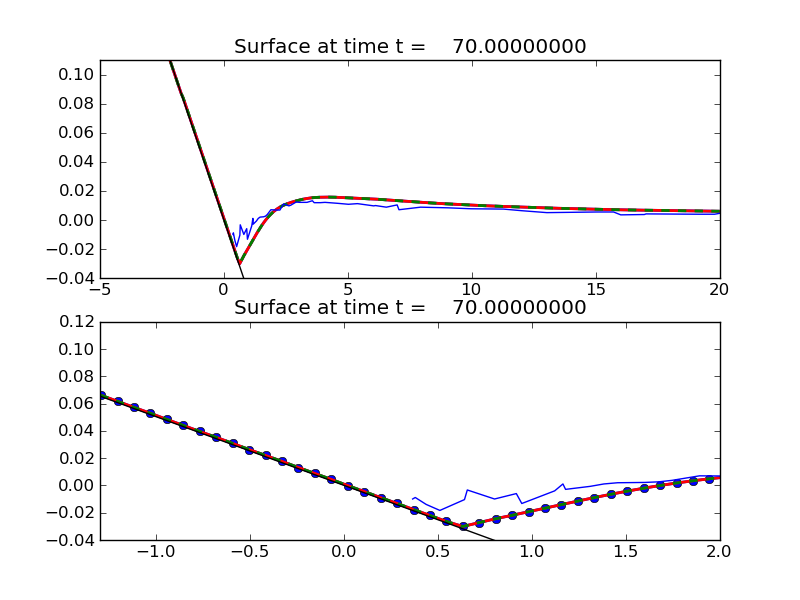
\includegraphics[width=2.8in]{../bp02/canonical-beach-lab-185/_plots/frame0005fig2.png}\hfil
\caption{\label{fig:bp2framesa} 
Frames of runup for low amplitude case. Top frame: Full view of incoming wave. Bottom Frame: Zoomed view of inundation area.}
\end{figure}

\begin{figure}[ht]
\hfil\includegraphics[width=2.8in]{../bp02/canonical-beach-lab-3/_plots/frame0001fig2.png}\hfil
\hfil\includegraphics[width=2.8in]{../bp02/canonical-beach-lab-3/_plots/frame0002fig2.png}\hfil
\vskip 5pt
\hfil\includegraphics[width=2.8in]{../bp02/canonical-beach-lab-3/_plots/frame0003fig2.png}\hfil
\hfil\includegraphics[width=2.8in]{../bp02/canonical-beach-lab-3/_plots/frame0004fig2.png}\hfil
\caption{\label{fig:bp2framesb} 
Frames of runup for high amplitude case. Top frame: Full view of incoming wave. Bottom Frame: Zoomed view of inundation area.}
\end{figure}

\subsection{Lessons learned}

\todo{This problem was a good physical verification of the framework developed in BP01. The low amplitude case had, as expected, a high degree of concurence with the predicted model. The higher amplitude case had a much lower degree of concurrence. This may be due to the steep shock that forms, requiring more complicated numerical modeling than that provided by the shallow water wave equations.}